Given a system that follows the VTS, we are interested in its connectivity (graph) property. We have implemented the encoding of the constraints in the python interface of $\zthree$. The basic idea is to constraint the variables such that vesicular transport rules are respected and using constraints (D0-D5) reason about the connectivity of the underlying structure (graph).

% We are interested in both least connectivity requirement (LRC) and least guarantee connectivity (LGC).
%LCR, that is required for a vesicular transport version to work and least connectivity that guarantees that vesicular transport system with that connectivity will always satisfies the rules.

% Whether a valid vesicular transport system is of certain connectiviity.   
%negation of the property .... STATE THE MEANING OF RESULT.  

%Besides using the default Z3 solvers we have used for these experiments \ankit{Z3, picoSAT, Lingeling}. The performance of Z3 was ...
%
% \Ankit{In other solver variations ...}
Our tool allows the user to choose a model and the size of the network besides other parameters like connectivity and number of parallel edges. It uses Z3 Python interface to build the needed constraints and applies $\zthree$ solver on the constraints to find a model ( a satisfying assignment that respects the constraints). This tool also translates the satisfying model found by $\zthree$ into a vesicle traffic system and presents a visual output to the user in form of annotated graph. The output graph will satisfy the underlying rules of the system, so it always is a valid vesicle transport network. The resultant graph provides an overview of the underlying vesicle transport system where directed labeled edges and nodes provide the complete information about the system. Dashed lines are used in the resultant visual network output to specify the dropped edges to make the graph disconnected, which gives information about the connectivity of the graph.

\begin{table}[t]
  \centering
  \begin{tabular}[t]{|c|c|c|c|c|}\hline
    Size & Model & Connectivity &Formula building (in secs) & Solver (in sec) \\\hline
  \end{tabular}
  \caption{Runtimes for searching for models}
  \label{tab:qf-grabh}
\end{table}
  \todo{Make table for all sizes and variants of the tool}

%--------------------- DO NOT ERASE BELOW THIS LINE --------------------------

%%% Local Variables:
%%% mode: latex
%%% TeX-master: "main"
%%% End:

%\begin{table}[t]
  \centering
  \begin{tabular}[t]{|c|c|c|c|c|c|c|c|c|}\hline
    {\multirow{2}{*} \textbf{Size}}  & \multicolumn{2}{c|}{\textbf{Variant A}} & \multicolumn{2}{c|}{\textbf{Variant C}} & \multicolumn{2}{c|}{\textbf{Variant D}}  &  \multicolumn{2}{c|}{\textbf{Variant F}} \\\hline
   
   \cline{2-9}
    {} & {\textbf{Z3}} & {\textbf{CBMC}} & {\textbf{Z3}} & {\textbf{CBMC}} & {\textbf{Z3}} & {\textbf{CBMC}} & {\textbf{Z3}} & {\textbf{CBMC}} \\\hline
    
    2 & !0.085 & !2.43 & 0.15 & 2.12 & !0.13 & !1.89 & 0.35 & 5.12 \\\hline
    3 & !0.54 & !8.04 & 0.95  & 7.65 & 0.62 & 7.66  & 1.36 & 23.94\\\hline
    4 & !2.57 & !297.93 & 2.33 & 22.74 & 2.85 & 48.35  & 4.81 & 123.34\\\hline
    5 & !7.7 & !3053.8 & 7.60 & 500.03 & 10.27 & 890.84 & 33.36  & 2482.71 \\\hline
    6 & !22.98 & M/O & 19.52 & M/O & 30.81 & M/O  & 147.52 & M/O\\\hline
    7 & !57.07 & M/O & 81.89 & M/O & 82.94 & M/O & 522.26  & M/O \\\hline
    8 & !164.14 & M/O & 630.85 & M/O & 303.19 & M/O & 2142.76 & M/O\\\hline
    9 & !307.67 & M/O & 2203.45 & M/O & 971.01 & M/O & 4243.34 & M/O\\\hline
    10 & !558.34 & M/O & 7681.93 & M/O & 2274.30 & M/O & 7786.82 & M/O\\\hline
  \end{tabular}
  \caption{Run-times for searching for models (in secs).}
  \label{tab:qf-grabh}
\end{table}


%   \begin{tabular}[t]{|c|c|c|}\hline
%    \textbf{Size}  & {\textbf{Model B}}  &  {\textbf{Model E}} \\\hline
%    
%    2 & !0.09 & !0.12 \\\hline
%    3  & !0.54  & !0.75 \\\hline
%    4 &  !2.33 & !3.35 \\\hline
%    5 & !7.7 & !13.05 \\\hline
%    6 &  !20.05 & !40.64 \\\hline
%    7 & !51.86 & !152.78 \\\hline
%    8 & !112.24 &  !344.26 \\\hline
%    9 &  !236.31 & !880.73\\\hline
%    10 &  !531.56 &  !2133.89\\\hline
%  \end{tabular}
%  \caption{Run-times for searching for models (in secs).}
% % \label{tab:qf-grabh}
%\end{table} 

%\begin{table}[t]
%  \centering
%  \begin{tabular}[t]{|c|c|c|c|}\hline
%    \textbf{Size} &  \textbf{Model A}   & \textbf{Model B} &  \textbf{Model E} \\\hline
%   
%    2 & !0.0853381156921 & !0.091157913208 & !0.117037057877 \\\hline
%    3 & !0.540871858597 & !0.537098646164  & !0.754279375076 \\\hline
%    4 & !2.57536292076 & !2.33045578003 & !3.35159707069 \\\hline
%    5 & !7.70005106926 & !7.71436476707 & !13.0516757965 \\\hline
%    6 & !22.9898321629 & !20.0573630333 & !40.6696507931 \\\hline
%    7 & !57.0719909668 & !51.860738039 & !152.783704758 \\\hline
%    8 & !164.140100718 &  !112.248553038 &  !344.268831253 \\\hline
%    9 & !307.675467253 & !236.317871094 & !880.730427027\\\hline
%    10 & !558.342684269 &  !531.565055132 &  !2133.8986\\\hline
%  \end{tabular}
%  \caption{Runtimes for searching for models}
%  \label{tab:qf-grabh}
%\end{table}

%--------------------- DO NOT ERASE BELOW THIS LINE --------------------------

%%% Local Variables:
%%% mode: latex
%%% TeX-master: "main"
%%% End:

In Table 1. 
%~\ref{tab:qf-graph},
we present the running times for the search of vesicle traffic systems of sizes 2 to 10 that satisfies the model variants. For example, the formula for variation F, the total number of compartments (N) equals to 10, returns in 129.78 minutes (7786.8 secs) with a SAT result. In comparison, CBMC encoding results in OUT OF MEMORY for the same variation and same compartment size. Hence with the use of this novel encoding, we are able to scale the system to a much larger compartmentalized system, especially to eukaryotic cells with a total number of ten compartments. This additional cushion of scalability can provide us leverage to ask for related open questions that were not previously possible, for example, what is the minimum number of molecules required to satisfy the vesicular traffic system in eukaryotes.

\begin{figure}[t]
  \centering
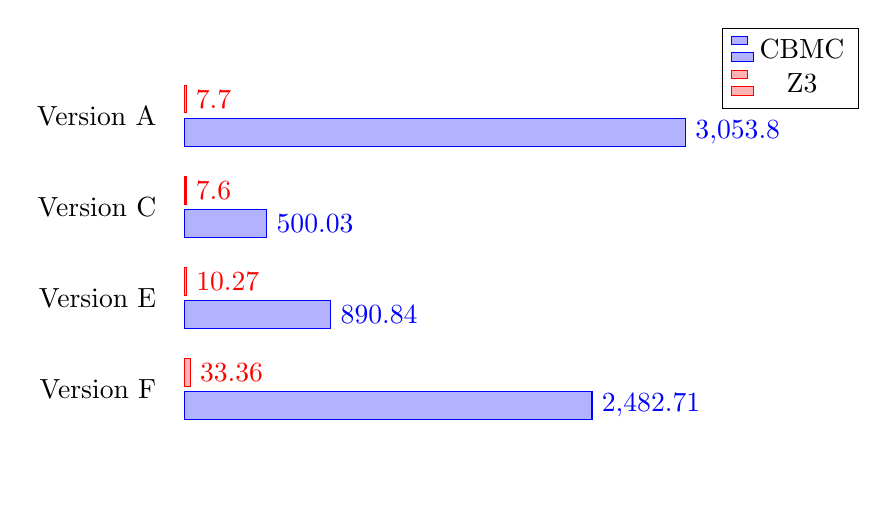
\begin{tikzpicture}
  \begin{axis}[
    xbar,
    y axis line style = { opacity = 0 },
    axis x line       = none,
    tickwidth         = 0pt,
    enlarge y limits  = 0.32,
    enlarge x limits  = 0.04,
    symbolic y coords = {Version F, Version E, Version C, Version A},
    nodes near coords,
    legend pos=outer north east,
  ]
  \legend{CBMC, Z3}
  \addplot coordinates { (3053.8,Version A)         (500.03,Version C)
                         (890.84,Version E)  (2482.71,Version F) };
  \addplot coordinates { (7.7,Version A)         (7.60,Version C)
                         (10.27,Version E)   (33.36,Version F)  };  
  \end{axis}
\end{tikzpicture}  
  \caption{CBMC Vs Z3 encoding for N $\equal$ 5 (in secs)}
  \label{fig:cz-comp}
\end{figure}

%%% Local Variables:
%%% mode: latex
%%% TeX-master: "main"
%%% End:


% REQUIRE COMPARISION WITH CBMC RUN TIME ?
The experiments were done on a machine with Intel(R) Core(TM) i3-4030U CPU @ 1.90GHz processor and 4GB RAM. On this machine, the CBMC encoding ran out of memory (M/O) for N $\geq$ 6 whereas new novel encoding was able to handle the case fairly easily. We think the main reasons for such an improvement are the following:
\begin{enumerate}
\item Direct encoding into the solver rather than using CFE (CBMC C front end), which treats front end variables as C variable and similarly other C overheads.
\item Current novel encoding is fine-tuned to the structure of the problem.
\item Improved encoding based on reachability rather than complete enumeration and non-determinism.
\end{enumerate} 
% 
$\zthree$ was able to solve the constraints up to 14-18 nodes (based on the versions).
%

%table~\ref{tbl:qf-results} 

\begin{table}[!ht]
\centering
\def\arraystretch{1.6}
\caption{
{\bf Activity regulation of molecules and corresponding connectivity of the graph.}}
  \begin{tabular}{|c|c|c|c|}
    \hline
  {\multirow{2}{*}{\textbf{Version}}}  & {\multirow{2}{*}{\textbf{Constraints}}} &  \multicolumn{2}{c|}{\textbf{Graph connectivity}}  \\
    % \hline
    % \textbf{Inactive Modes} & \textbf{Description}\\
   \cline{3-4}
   {} & {} & \textbf{\textbf{Least connected}} & \textbf{Sampling: Guarantee}\\
    %\hhline{~--}
    \hline
    
%    A. & V1-V7 V8 V9 R1 R2 D1-D4 A\_nn A\_en & No graph  \\ \hline
%B. & V1-V7 V8 V9 R1 R2 D1-D4 A\_nb A\_en & No graph  \\ \hline
%C. & V1-V7 V8 V9 R1 R2 D1-D4 A\_nn A\_eb & 3-connected  \\  \hline
%D. & V1-V7 V8 V9 R1 R2 D1-D4 A\_nn A\_ep & No graph  \\ \hline
%E. & V1-V7 V8 V9 R1 R2 D1-D4 A\_nb A\_eb & 2-connected  \\ \hline
%F. & V1-V7 V8 V9 R1 R2 D1-D4 A\_nb A\_ep & 4-connected  \\ \hline
%G. & V1-V7 V8 V9 R1 R2 D1-D4 A\_nb A\_eb C\_ed & 3-connected \\ \hline

A. & V1-V7 V8 V9 R1 R2 D1-D4 A\_nn A\_en & No graph & No graph \\ \hline
B. & V1-V7 V8 V9 R1 R2 D1-D4 A\_nb A\_en & No graph & No graph \\ \hline
C. & V1-V7 V8 V9 R1 R2 D1-D4 A\_nn A\_eb & 3-connected & 3-connected \\  \hline
D. & V1-V7 V8 V9 R1 R2 D1-D4 A\_nn A\_ep & No graph & No graph \\ \hline
E. & V1-V7 V8 V9 R1 R2 D1-D4 A\_nb A\_eb & 2-connected & 3-connected \\ \hline
F. & V1-V7 V8 V9 R1 R2 D1-D4 A\_nb A\_ep & 4-connected & 4-connected \\ \hline
G. & V1-V7 V8 V9 R1 R2 D1-D4 A\_nb A\_eb C\_ed & 3-connected & 3-connected \\ \hline
%H. & V1-V7 V8 V9 R1 R2 D1-D4 A\_nb  A\_eb + C\_es & No-idea & No-idea \\ \hline

% C_es :Self edges are allowed
% C_ed : Every edge is distinct 
  \end{tabular}
\label{table1}
\end{table}


%--------------------- DO NOT ERASE BELOW THIS LINE --------------------------

%%% Local Variables:
%%% mode: latex
%%% TeX-master: "main"
%%% End:
